% Generated once by scripts/paper_md2tex.py from docs/paper/draft.md; edit this file from now on.
\section{Symbolic studies in full}\label{app:E}
\noindent Record sections 5 to 7: the oracle and learned-writer mechanism experiments, the same-rank and historical budget controls, and the stopping studies.
\subsection*{5. Mechanism experiments: depth is useful under specific writing conditions}\addcontentsline{toc}{subsection}{5. Mechanism experiments: depth is useful under specific writing conditions}

We report candidate-restricted accuracy and distinguish percentage points (pp) from
absolute percentages. Confirmation intervals are 97.5\% paired episode-bootstrap  % S1 S9
intervals conditional on the three fixed training seeds; absolute point profiles
have no standalone confidence intervals. The depth  % S1 S3 S9
effect D is L4 minus L1 on hops2-3; walk specificity W subtracts the corresponding
effect on far hops6-8. This subtraction prevents a generic all-hop shift from being
described as selective improvement on the trained reachable hops. How far D measures
composition rather than escape from a neighbour error is qualified in Section 6.
% PM1

The primary protocol treats reach, specificity, preservation of the single-hop task,
and replication as separate requirements; an improvement on only the reachable-hop
average is insufficient for its full gate.  % S1 S4 S5 S9
The fixed-query comparison addresses a different alternative explanation: internal
iterations may help even when the context observation is cached. The memory-free
comparison asks whether those iterations need any stored context at all. Neither
control is replaced by a larger-rank comparison, which changes the representation
budget. These distinctions explain why we retain both the registered composite
outcome and its component contrasts instead of selecting whichever metric is most
favorable for a particular writer.

The primary stage and its follow-ups also differ in evidential strength. The
original stage includes the registered changed-layout replication, whereas the
rank and factorized follow-ups report their own unreplicated results on the
reused confirmation set. For learned  % S1 S5 S8 S9
writers, a within-checkpoint depth contrast fixes that checkpoint’s writer and
memory; a comparison of reader variants generally does not fix the jointly
trained writer. We consequently interpret depth effects,  % S3 S9
control effects, and cross-writer differences separately. A figure showing one
checkpoint helps expose the depth trajectory, but it cannot replace the pooled
endpoint or its training-seed breakdown.

\subsubsection*{5.1 Oracle writing and controlled reader contrasts}

With orthogonal oracle writing, r32 M1 has D=+92.883 pp [92.233, 93.550] and
W=+92.872 pp [92.208, 93.564] on confirmation seed777001, while also improving hop1.
 The separately trained evolving-query reader exceeds B5 by +92.892 pp  % S1
[92.150, 93.542] and B3 by +85.233 pp [84.233, 86.183] on hops2-3 at L4, using the
same primary oracle codebook. These contrasts support repeated,  % S2
query-dependent memory use for the tested task, rather than an explanation solely
in terms of more memory-free iterations.  % S1 S2

Exact one-hop-per-read timing is nevertheless not an empirical result.  % S7
For the trained orthogonal M1-lin reader, hop4 accuracy at L4 is 2.483\%, and hop8 at
L8 is zero, despite high accuracies for some intermediate longer hops at L8.  % S7
Its hop1 accuracy falls from 99.567\% at L1 to 96.550\% at L4 and 26.300\% at L8.
 These cells reject the automatic identification of a trained reader with  % S7
Proposition 3’s aligned construction; they do not refute its sufficient conditions.
 The apparent benefit of depth must be described by hop and evaluation  % S7
depth, including the short-hop losses.

Random oracle codes give a different balance. At r32, M1 improves reachable hops by
+33.258 pp [32.016, 34.484] but loses 18.933 pp on hop1; M1-lin likewise has a positive
depth effect and a substantial hop1 loss. Both conditions fail only the  % S6
hop-preservation criterion. Random oracle codes therefore should not be  % S6
treated as interference-free storage, and their positive reachable-hop effect should
not be relabeled a full gate pass.  % S6

\begin{figure}[htbp]
\centering
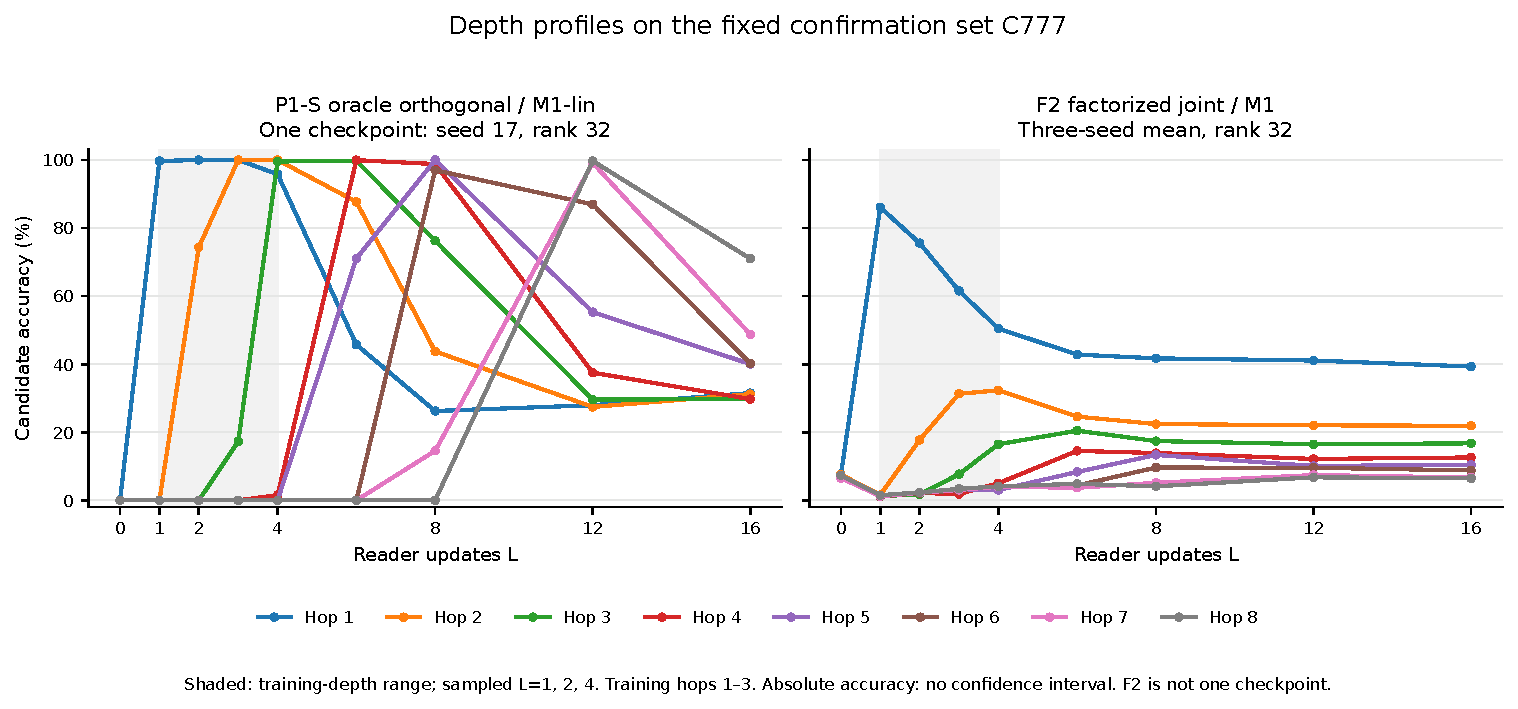
\includegraphics[width=0.96\linewidth]{../figures/quality_depth.pdf}
\caption{Quality versus evaluation depth by hop: P1-S oracle\_orth/\allowbreak{}M1-lin uses the
individual seed17 checkpoint; F2 joint\_fact/\allowbreak{}M1 uses the three-seed mean of fixed-checkpoint
sweeps because individual-checkpoint F2 cells are not committed. Candidate-restricted  % S7 S9
accuracy, confirmation seed777001; source selectors are recorded with the figure.  % S7 S9
Curves have no confidence bands and do not imply exact one-hop timing or hop preservation.
% S7 S9
}
\end{figure}

\begin{figure}[htbp]
\centering
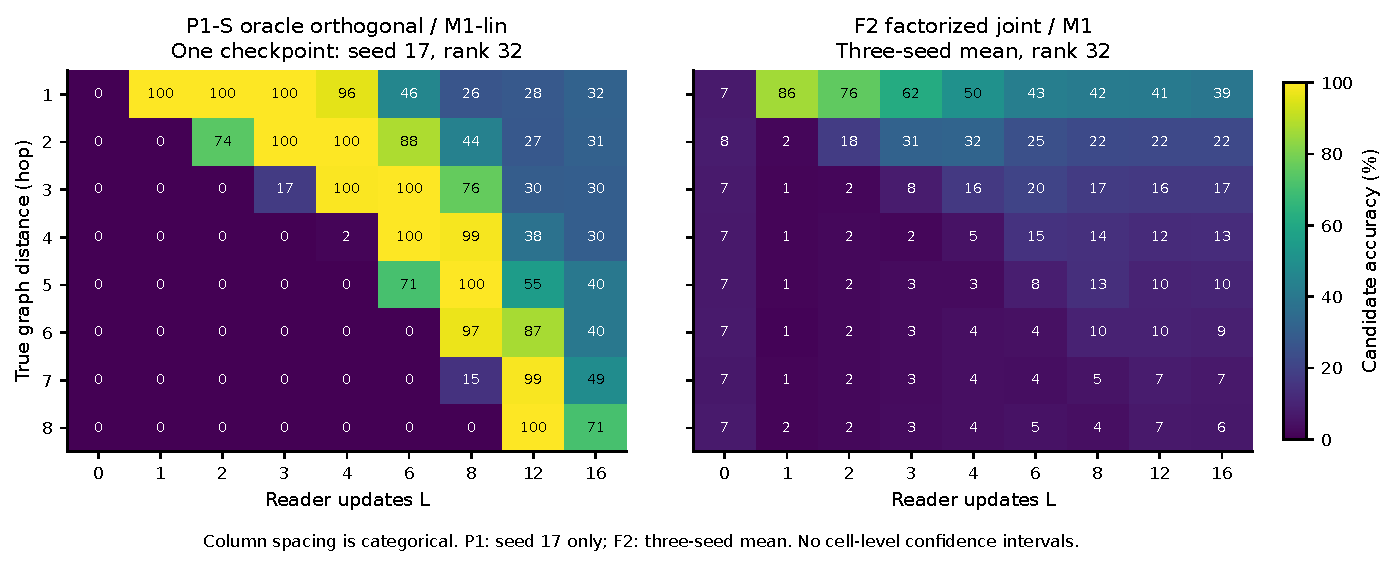
\includegraphics[width=0.96\linewidth]{../figures/hop_depth_heatmap.pdf}
\caption{Hop\ensuremath{\times}L views of the same committed conditions: the left panel is seed17,
and the right panel is the three-seed mean, as in Figure 1. Training hop lengths and  % S7 S9
evaluation depths must be distinguished when reading extrapolation cells; successful
individual cells do not establish uniform longer-hop success.  % S7 S9
}
\end{figure}

\subsubsection*{5.2 Learned writers, factorization, and seed dependence}

The unfactorized joint r32 M1 condition passes the registered gate with a much
smaller effect: D=+8.292 pp [7.383, 9.292] and W=+2.492 pp [1.244, 3.733].  % S3
Its mean advantage over B5 is +7.767 pp [6.516, 9.050], but the three seed effects
are +9.300, \ensuremath{-}17.700, and +31.700 pp. The pooled interval is consequently  % S3
compatible with a failed training seed, and it does not establish improvement for a
population of new seeds. The joint linear reader fails the primary depth  % S3
gate, with specificity \ensuremath{-}0.408 pp [\ensuremath{-}1.475, 0.753].  % S4

Unfactorized frozen T1 writers fail the replication-specificity criterion for both
readers; the M1 replication interval includes zero. This result does not  % S5
show that joint training is necessary for every composable writer, because factorized
frozen writers produce positive depth and specificity effects under the tested F2
protocol. Even the matched factorized T1 sources' validation  % S5 S9
accuracies above 91\% do not certify the full T2 gate after freezing: the resulting
readers retain positive depth effects but fail hop1 preservation.  % S12 S9

Factorization makes the distinction between composition evidence and overall utility
particularly clear. On the reused confirmation set C777, joint\_fact M1 yields
D=+22.975 pp [22.017, 23.975] and W=+20.158 pp [19.058, 21.192], but H=\ensuremath{-}35.617 pp
[\ensuremath{-}37.217, \ensuremath{-}33.933]. All  % S9
four factorized writer/\allowbreak{}reader conditions fail the complete depth gate because of
hop1 loss, even though their reach, specificity, and control contrasts pass the
reported criteria. Moreover, joint\_fact M1’s final L4 reachable-hop  % S9
contrast against the unfactorized joint system is \ensuremath{-}19.108 pp [\ensuremath{-}20.534, \ensuremath{-}17.600],
despite a larger depth contrast. Improving a contrast from a weaker  % S10
L1 baseline is therefore not equivalent to improving the deployed L4 system.
% S10

The larger-rank follow-up gives stronger joint-code effects in its tested regimes:
r64 M1 has D=+30.533 pp [29.225, 31.900], and its B5 contrast is +24.017 pp
[22.575, 25.575] pooled, with seed effects +22.575, +25.075, and +24.400 pp.  % S8
However, rank and training steps are confounded: it uses 20,000 training steps instead
of the primary study’s 15,000, and has no replication, so the comparison cannot isolate
rank or establish new-seed robustness. Its evaluation also reuses the C777 confirmation
set after P1-S, so its intervals are not an independent confirmation.  % S8

\begin{figure}[htbp]
\centering
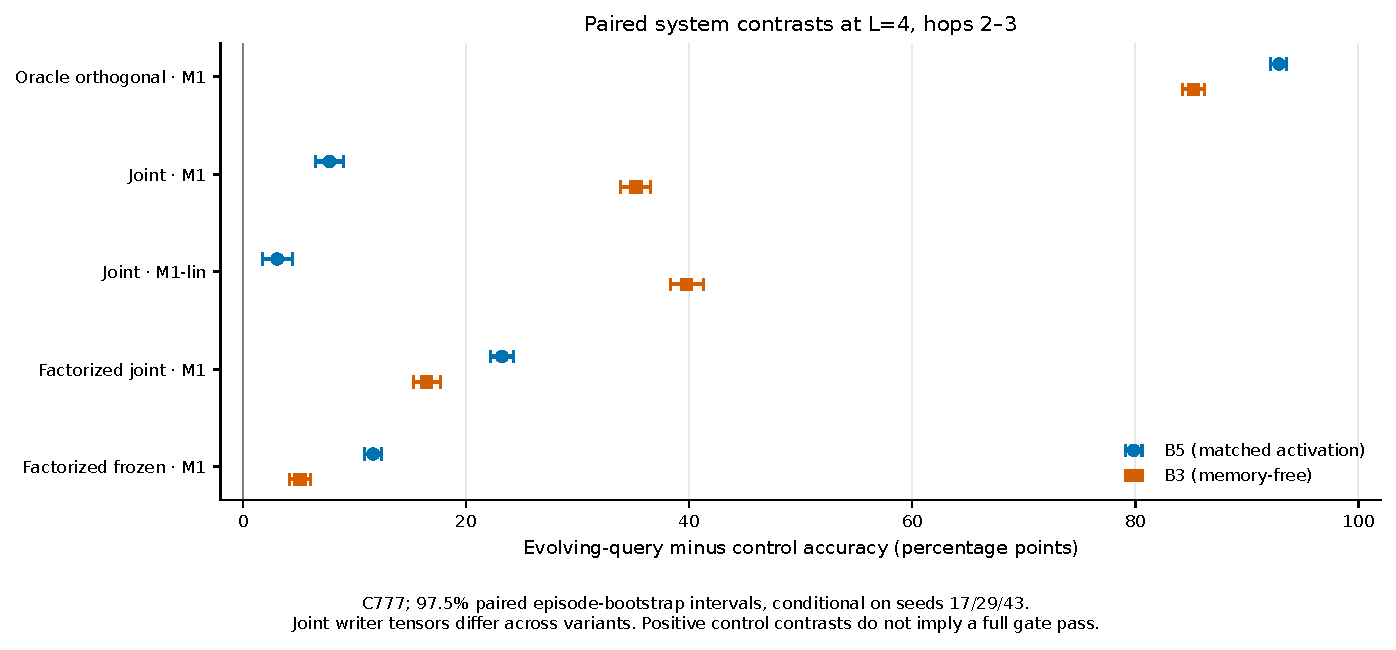
\includegraphics[width=0.96\linewidth]{../figures/paired_controls.pdf}
\caption{Paired hops2-3 contrasts at L4 against fixed-query B5 and memory-free B3;
displayed intervals are the released 97.5\% episode-bootstrap intervals. Oracle and  % S2 S3 S9
learned writer conditions must retain their different sharing controls, and positive
pooled effects do not require every training seed to improve.  % S2 S3 S9
}
\end{figure}

\subsubsection*{5.3 Counterfactual specificity and decision history}

Successor swaps provide screening-only diagnostics without released confidence
intervals. For joint M1 at L4, among the  % S11
specified P1-S rows whose new path fits, the new-terminal follow rate is 44.220\%
versus 35.293\% for the unswapped query; joint M1-lin is nearly unchanged at
48.336\% versus 47.913\%. The factorized M1 new-path-length-one stratum  % S11
has 47.985\% versus 4.426\%, but that different stratum prevents interpreting the
cross-study rate difference as a controlled factorization effect.  % S11
These responses are consistent with path-sensitive behavior without uniquely
identifying pointer chasing or excluding global terminal statistics.  % S11

The continuation decision also needs disclosure. The evidence ledger’s
decision-history correction, item 4 records an
explicit deviation from F2’s original no-go rule: the orchestrator continued toward
P1-L using the earlier joint/\allowbreak{}M1 pass, while using F2 to inform writer form.  % S3 S9
This decision did not turn the factorized failures into passes. It belongs  % S9
in the interpretation of the study, because a preregistered gate and a later justified
continuation decision are different records.


\subsection*{6. Same-rank comparisons, reported costs, and historical budget controls}\addcontentsline{toc}{subsection}{6. Same-rank comparisons, reported costs, and historical budget controls}

The primary baseline is the single read at the same rank, so the shared-reader
comparison changes computation depth without increasing parameter count. With an  % FR1
otherwise identical architecture, shared M1-L4 and B4 have exactly the same parameter
count, and “equal parameters” is reserved for that pair. B8 is not  % FR1
parameter-matched to either: its step-specific R/\allowbreak{}U/\allowbreak{}Q add 3(r\ensuremath{^2}+2r\ensuremath{\cdot}r\_mem) parameters,
9,216 at r=r\_mem=32 and 147,456 at r=r\_mem=128. The registered P1-L adapter  % FR1
counts are 103,426 becoming 112,642 at rank32 (+8.9\%) and 475,138 becoming 622,594 at
rank128 (+31.0\%); in the symbolic unfactorized joint model the counts are 13,314 becoming
22,530 (+69.2\%). Each percentage belongs to its own model; none is the  % FR1
proportion of trainable oracle parameters or a whole-backbone figure. Extra  % FR1
reader latency is reported as a cost of the additional computation.  % FR1

\subsubsection*{Historical rank, state, and sharing controls}

P2-S compares r32 shared M1 at L4 with larger single reads and an unshared reader on
confirmation set C888; the reference M1 uses mixed-depth training, while B6/\allowbreak{}B7 train at
L1 and B8 (+9,216 parameters, not parameter-matched) at fixed
L4. With unfactorized joint writing, M1  % B1 B2 B3 B4
beats B6/\allowbreak{}r64 on reachable hops by +14.875 pp [13.658, 16.184] pooled, but the three seed
effects are +33.125, \ensuremath{-}20.675, and +32.175 pp, so seed29 is negative. The M1\ensuremath{-}B6/\allowbreak{}r128 contrast is \ensuremath{-}3.233 pp  % B1
[\ensuremath{-}4.675, \ensuremath{-}1.833], and M1 also scores below both larger-state B7 configurations. Thus the claim  % B1
that these larger single reads cannot replace the tested joint system is not
supported. With random oracle codes, by contrast, M1 exceeds B6/\allowbreak{}r64  % B1
and r128 by +34.750 and +34.775 pp, respectively, with positive intervals and positive
effects in every tested seed.  % B2

The factorized follow-up, which reuses the P2-S confirmation set C888, also supports a
bounded capability claim. Mixed-depth
joint\_fact M1/\allowbreak{}r32 at L4 exceeds B6/\allowbreak{}r64, B6/\allowbreak{}r128, B7/\allowbreak{}r\_mem64, and B7/\allowbreak{}r\_mem128 by
+24.017, +24.242, +23.875, and +23.550 pp, respectively; every reported interval
and tested-seed effect is positive. These are comparisons against the  % B5
specified trained architectures, not an information-theoretic ceiling for every
single-read function.  % B5

On the primary E12 layout the uniform-candidate chance level is 1/\allowbreak{}14\ensuremath{\approx}7.1\%. The single
reads in these comparisons score far below it on reachable hops: 0.025\% and 0.000\% for
B6/\allowbreak{}r64 and r128 under random oracle codes, and 0.242-0.933\% for the larger single reads
under factorized joint writing. The frozen-writer factorized M1 at  % B2 B5
L1 shows the same pattern, at 1.983\% on hop2 and 1.033\% on hop3. Accuracy far  % S12
below chance indicates systematic errors rather than uninformed guessing. One candidate
explanation is that a single read tends to return the one-hop neighbour of the queried
entity, in which case part of a depth effect would be escape from that error rather than
composition. \textbf{Neighbour-confusion rate.} NCR categorises the wrong hop2 answers of the
single read (L1) of released M1 and of B4, from the saved screening (S4242) and confirmation
(C777) predictions of the existing r32 P1-S and F2 runs, with descriptive 95\% intervals. In the
16 groups whose hop2 accuracy is below the 7.143\% chance line (t1\_frozen\_fact, joint\_fact,
oracle\_random and oracle\_orth, each with M1 and B4 on both sets), the share of errors that
name the one-hop neighbour is 58.667-100.000\%, against 7.692\% for a uniform wrong guess, and
every interval lower bound exceeds the uniform value. The share is 89.739-100.000\%  % PM1
for B4 and 58.667-87.159\% for M1, while the unfactorized joint and t1\_frozen writers read above
chance at hop2 with first-hop shares of 5.3-23.0\%. A share above  % PM1 NC2
its uniform value says that the single read returns the neighbour more often than a uniform error
would; it does not identify the mechanism. The tables qualify the reading of D  % PM1
only: in the groups below chance, part of the L4\ensuremath{-}L1 gain on hops2-3 may measure escape from
the neighbour error rather than composition, and because the errors at L4 are not categorised,
no fraction of D is estimated.  % PM1

The two kinds of positive result should not be combined into an unrestricted resource
claim. A fixed-rank depth sweep spends more reader operations at the same persistent
state size. A larger-rank single read changes both its representational width and
state storage, while a larger-memory comparison changes the state while retaining the
same reader width. Each comparison rules out a different explanation for the observed  % B1 B5
accuracy; none licenses replacing measured latency by an analytic operation count.
The current factorized result establishes only the tested capability contrast, with
its accuracy-latency frontier still unmeasured.  % B5 B8

Matching training depth narrows the sharing question. On the reused set C888, B8 minus
shared M1-L4 has reachable-hop effects of +13.217 pp [11.983, 14.450] for joint writing,
+5.458 [4.242, 6.750] for joint\_fact, and +3.200 [1.958, 4.517] for random oracle
writing, each positive in every tested seed. This comparison also changes parameter count and, for learned  % B3
joint writing, writer parameters; it is not a parameter-neutral causal estimate
of sharing. B8 is not parameter-matched to M1-L4: the joint model has 22,530 versus
13,314 parameters (+9,216, +69.2\%), and oracle\_random has 16,386 versus 7,170 registered
and 13,312 versus 4,096 trained parameters (+128.5\% and +225.0\%); joint\_fact totals are
not recorded. Fixed-L4 shared training improves over the mixed-depth  % B3 FR1
reference, reducing the joint B8 gap from 33.733 to 13.217 pp, but the selected
protocol comparison does not identify a unique causal fraction due to depth.
 B8’s pooled long-hop accuracy at evaluation L4 is lower for all three  % B4
writers, so its trained-hop advantage is not evidence of superior depth extrapolation.
% B6

Under P2-S’s original registered practical criterion, the result is negative. Joint M1/\allowbreak{}r32 at L4 attains 48.017\% hops1-3 accuracy  % B7
at 0.848 ms per prepared batch64, whereas joint B6/\allowbreak{}r128 at L1 attains 57.244\% at
0.352 ms; these are descriptive CUDA-event means without timing intervals.  % B7
Every eligible joint M1 depth point is matched by an equal-or-faster single-step
point for both tested batch sizes, and Gate 3 fails. Those models spend  % B7
different parameter and state budgets, so the negative practical result does not
erase the fixed-budget composition contrast; it rejects a broader efficiency claim.
 P2-S-F1 supplies no factorized accuracy-latency benchmark.  % S3 B7
 This historical measurement gap is not converted into an efficiency  % B8
claim, and the same-rank design does not relabel the earlier gate.
% B7 FR1

The parameter and storage differences make the intended tradeoff concrete: the
joint M1 point has 13,314 trained parameters and 4,096 persistent FP32 bytes per
episode, versus 114,690 parameters and 65,536 bytes for B6/\allowbreak{}r128. A  % B7
reader may therefore be attractive under a strict state allocation even when it
does not win the measured latency comparison. That possible application is a
conditional design choice, not a practical advantage established for the full
request path. The reported timings exclude the context writer and other preparation,
and the follow-up’s aggregate resource ledger cannot supply missing comparative
training costs for individual models.  % B7 B8

\begin{figure}[htbp]
\centering
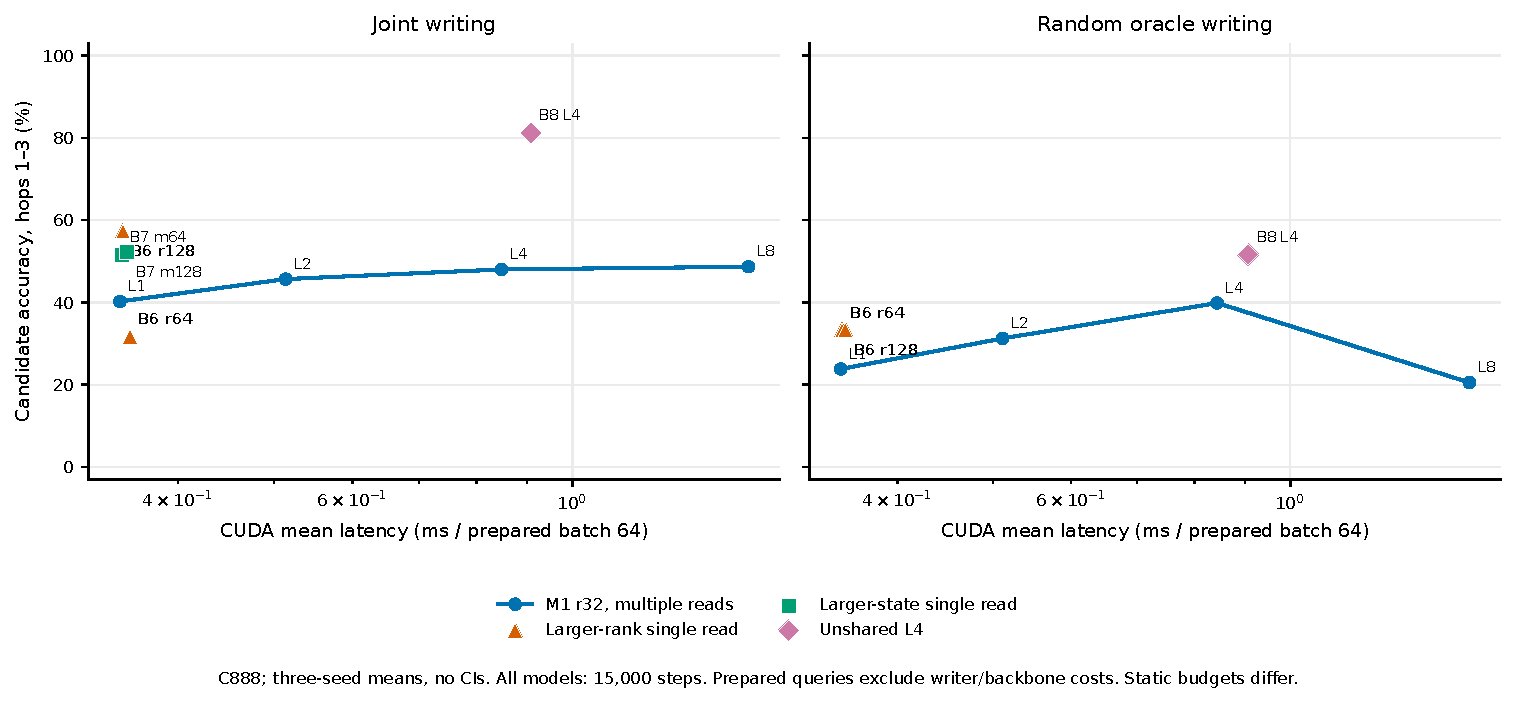
\includegraphics[width=0.96\linewidth]{../figures/budget_latency.pdf}
\caption{P2-S accuracy-latency points, with larger-rank single reads marked.  % B7
Accuracy averages hops1-3, rather than only the reachable-hop endpoint; timings
exclude writer/\allowbreak{}context preparation and are descriptive means. Different ranks trade  % B7
different parameters and persistent-state budgets.  % B7 B8
}
\end{figure}

\subsubsection*{Memory load, adaptation, and updated facts}

Study IS uses a new confirmation set, C999 (evaluation seed999001, 2,000 episodes
per load), at r=r\_mem=32, with oracle\_random and joint\_fact as primary writers.
 Its fixed E12-trained M1 checkpoints are evaluated at  % IS1 IS2
E6/\allowbreak{}12/\allowbreak{}18/\allowbreak{}24/\allowbreak{}36; increasing load also changes chain layout and candidate count.
 D(E) compares L4 with L1 on reachable hops2-3 within each checkpoint.  % IS1
For oracle writing, D falls from 34.750 pp at E12 to 7.492 pp at E36, with
DeltaD=\ensuremath{-}27.258 pp [\ensuremath{-}28.800, \ensuremath{-}25.816]; for factorized writing it falls from
24.042 to 4.642 pp, with DeltaD=\ensuremath{-}19.400 pp [\ensuremath{-}20.542, \ensuremath{-}18.241].  % IS1
Both changes are negative in every tested seed (seeds17/\allowbreak{}29/\allowbreak{}43: oracle\_random \ensuremath{-}28.725,
\ensuremath{-}25.900, \ensuremath{-}27.150 pp; joint\_fact \ensuremath{-}20.525, \ensuremath{-}19.200, \ensuremath{-}18.475 pp); their 97.5\% intervals use
independent load bootstrap streams rather than cross-layout episode pairing.  % IS1
This supports the registered operational load/\allowbreak{}depth prediction without identifying
crosstalk as its sole cause or validating Proposition 4’s operator bound as tight.
% IS1

IVD asks whether key interference explains this shrinkage, on the same frozen r32 M1
checkpoints and a new set C999004 (evaluation seed999004, 2,000 episodes per checkpoint). It
keeps the twelve-fact chains, queries, answers and the 14-entity candidate set fixed, adds up
to 24 extra facts whose heads lie outside the episode and whose tails lie inside it, and
varies the overlap of the extras' keys with the relevant keys at equal load. Its endpoint
is IC=G(low)\ensuremath{-}G(high) at load 24, where G is L4\ensuremath{-}L1 of M1 on hops2-3; a writer passes if
IC\ensuremath{\geq}5 pp and the lower bound of the 97.5\% interval is above 0. For  % IV1 IV2
oracle\_random, with constructed key codes, IC=+13.975 pp [12.642, 15.242] (seeds +14.850,
+13.250, +13.825 pp) and the achieved overlap gap is 0.500, so the shrinkage is consistent with
key interference, identified by IVD for oracle\_random. For joint\_fact, whose  % IV1
overlap is selected among candidate heads, IC=+3.208 pp [2.175, 4.208] is below the 5 pp
threshold (overlap gap 0.285): the paper does not offer interference as the identified
explanation of the IS shrinkage for joint\_fact, and states that load, graph layout and
candidate distribution were changed together in IS. At load 24 G is below the  % IV2
unmodified base cell in every cell, including low overlap (oracle\_random +25.542 pp at low
overlap against +33.092; joint\_fact +10.833 against +23.383), and a decay-only control leaves
joint\_fact’s G unchanged at +23.383 pp. The extras bring the stored facts to 18  % IV3
or 36, outside the readers' training distribution, and the constructed codes can themselves
be out of distribution; the result narrows the IS wording for one writer and does not make
interference the sole cause for either.  % IV1 IV2

\begin{figure}[htbp]
\centering
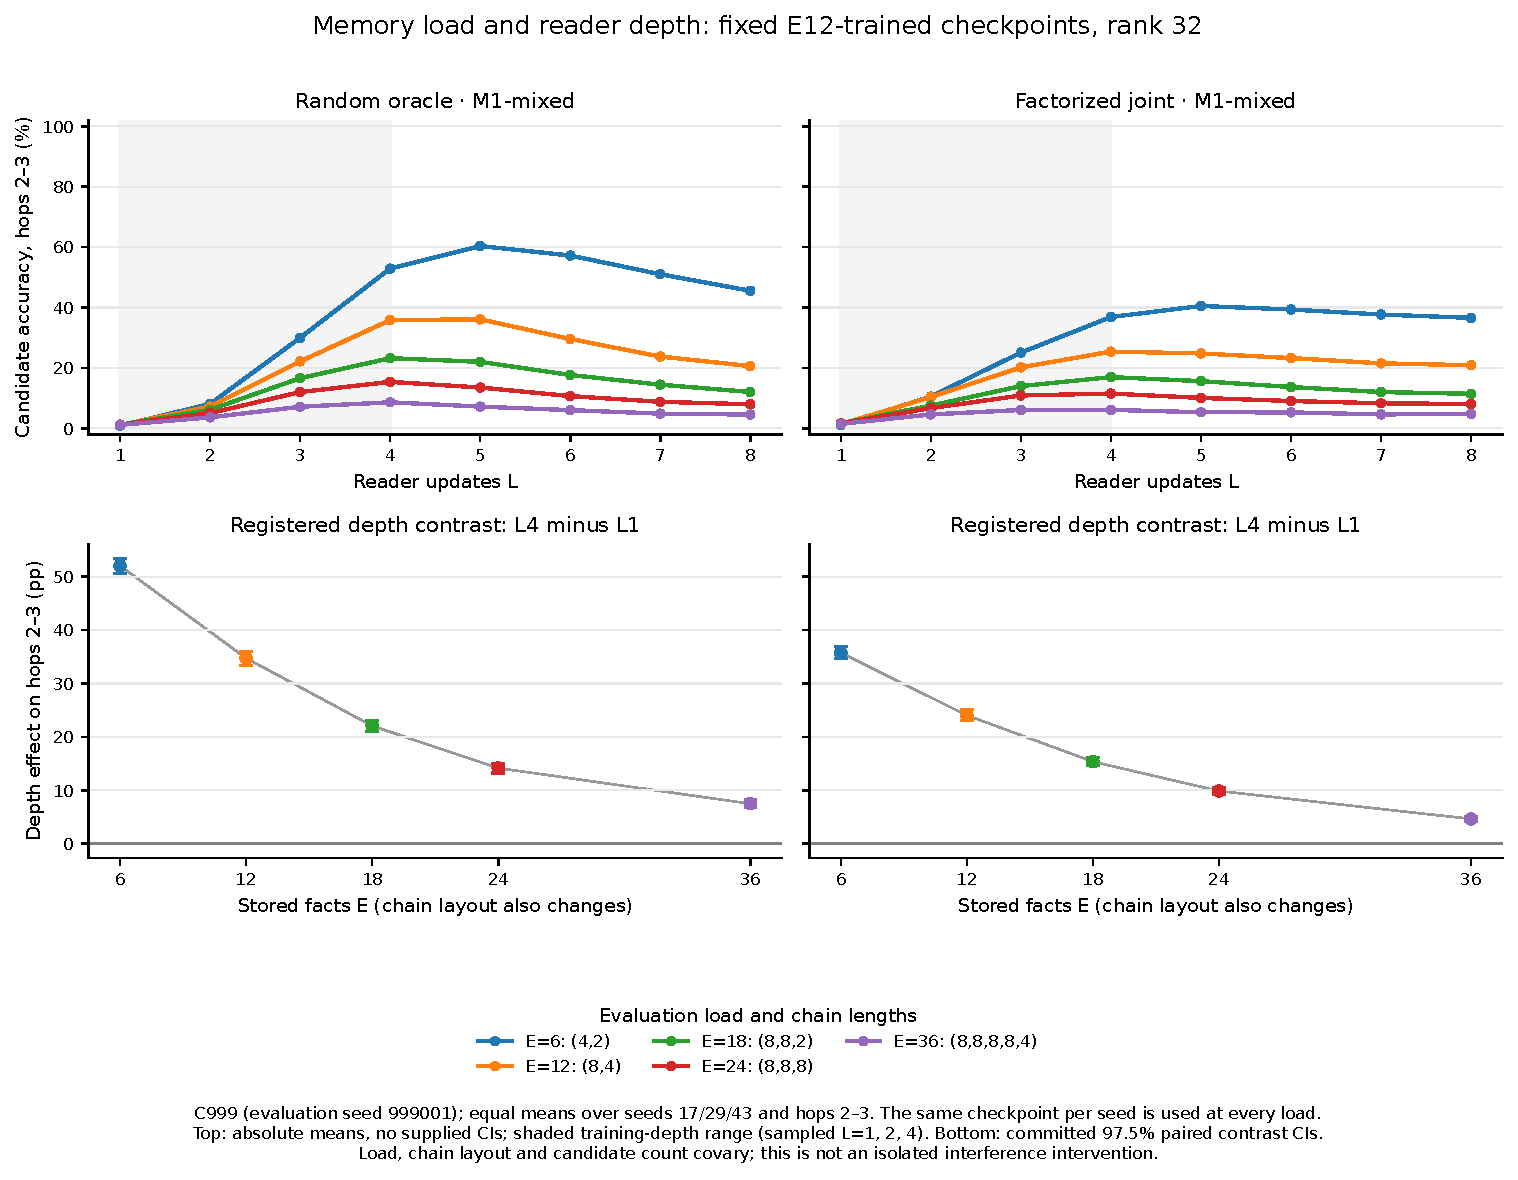
\includegraphics[width=0.96\linewidth]{../figures/memory_load_depth.pdf}
\caption{Plan \S{}9.3 item4: fixed E12-trained shared M1 checkpoints across load/\allowbreak{}layout
conditions, averaging seeds17/\allowbreak{}29/\allowbreak{}43 and hops2-3 on C999. Top panels show  % IS1
absolute accuracy means without supplied CIs; bottom panels reuse the released
97.5\% within-load L4\ensuremath{-}L1 intervals. The same checkpoint per seed is used  % IS1
at every load, while chain layouts and candidate counts covary.  % IS1
}
\end{figure}

For models trained at their evaluation load, all tested E12/\allowbreak{}24/\allowbreak{}36 M1@4 and B8@4
contrasts against B4@1 meet the registered point\ensuremath{\geq}3 pp and CI lower>0 rule, and all 36
tested-seed effects are positive. B8 adds 9,216 parameters, so it is not  % IS2
parameter-matched to B4 or M1; the percentage depends on the writer’s parameter count.
 At the largest tested load, E36, their reachable-hop margins are:  % FR1
% IS2


{\small
\setlength{\tabcolsep}{3pt}
\begin{longtable}{W{187}{6}W{363}{6}W{451}{6}}
\toprule
Writer & M1-mixed@4\ensuremath{-}B4@1, pp [97.5\% CI] & B8@4\ensuremath{-}B4@1 (B8 +9,216 parameters), pp [97.5\% CI] \\ \addlinespace[3pt]
\midrule \endhead
oracle\_random & +4.483 [3.950, 5.033] & +5.942 [5.225, 6.675] \\ \addlinespace[3pt]  % IS2 IS2
joint\_fact & +3.433 [2.983, 3.867] & +5.008 [4.500, 5.500] \\ \addlinespace[3pt]  % IS2 IS2
\bottomrule
\end{longtable}
}


The factorized M1 interval need not have its lower endpoint above 3 pp to qualify;
the threshold applies to the point estimate. These are separately trained  % IS2
systems with different depth/\allowbreak{}sharing conditions, not a recheck of hop1 preservation
or the practical latency gate; the capability failure boundary beyond E36 was not
located. Under the inherited learning rate and fixed-step  % IS2 B7
protocol, all eight load-specific E24/\allowbreak{}E36 training contrasts against E12-trained
models evaluated at the same load are negative, ranging from \ensuremath{-}6.283 to \ensuremath{-}2.042 pp,
with negative intervals and negative effects in all 24 seed-level contrasts. That result does not show that independently  % IS3
tuned or convergence-matched load adaptation is generally harmful.  % IS3

The update-task check uses unchanged E12-trained readers with 14 stored facts:
12 current edges plus two obsolete records; its pooled queries cover hops1-4.
 For B8@4 (+9,216 parameters, not parameter-matched to the shared readers;  % IS4
FR1), the absolute current/\allowbreak{}stale rates are:
% IS4


{\footnotesize
\setlength{\tabcolsep}{3pt}
\begin{longtable}{W{127}{8}W{285}{8}W{289}{8}W{299}{8}}
\toprule
Writer & Current, affected paths, \% [97.5\% CI] & Current, untouched paths, \% [97.5\% CI] & Obsolete terminal, affected paths, \% [97.5\% CI] \\ \addlinespace[3pt]
\midrule \endhead
oracle\_random & 41.750 [40.235, 43.300] & 37.606 [36.051, 39.211] & 0.510 [0.332, 0.712] \\ \addlinespace[3pt]  % IS4 IS4 IS4
joint\_fact & 28.619 [27.452, 29.735] & 30.468 [29.357, 31.648] & 6.035 [5.486, 6.591] \\ \addlinespace[3pt]  % IS4 IS4 IS4
\bottomrule
\end{longtable}
}


Current terminals are selected more often than obsolete ones in these primary B8
conditions, with partial overall success. These are absolute-rate  % IS4
intervals, not paired intervals for current\ensuremath{-}stale or affected\ensuremath{-}untouched effects;
untouched-path stale rates are undefined. They establish neither a  % IS4
causal benefit from updating nor a guarantee that every reader follows updated paths.
% IS4


\subsection*{7. Stopping and overshoot: post-hoc selection and training-time regularization}\addcontentsline{toc}{subsection}{7. Stopping and overshoot: post-hoc selection and training-time regularization}

\subsubsection*{Earlier screening policies}

The earlier label-free policies select thresholds using mean validation accuracy, freeze them,
and evaluate on screening seed4242 without confidence intervals; no confirmation
result is supplied for those pilots. Relative-change stopping on random-oracle  % H1 H4
r128 M1, from the 20,000-step rank-follow-up checkpoints where rank and training steps
are confounded, increases long-hop accuracy from 45.747\% at L8 to 70.690\%, using 8.301 mean
updates, but its hop1 accuracy remains below L1: 87.883\% versus 99.983\%.  % H1
The corresponding linear reader also improves long-hop screening accuracy while
retaining a hop1 loss. This is a selected empirical tradeoff, not a  % H1
certificate that the chain terminal has been reached.  % H1 H3

The tested r32 factorized stopping policies do not repair the hop1 preservation
failure. All 12 factorized  % H4
family/\allowbreak{}rule choices fail hop1 preservation; even each family’s descriptively
least-loss screening rule loses between 24.900 and 41.733 pp relative to L1.
 The unfactorized joint/\allowbreak{}M1 screening flag supplies no adaptive benefit  % H4
either: all three rules use exactly 16 mean updates and reproduce fixed-L16
endpoints, with a negative specificity effect in one training seed (minimum seed W
\ensuremath{-}0.125 pp).  % H5
These outcomes restrict the tested rules, rather than ruling out every possible
halting policy.  % H4 H5

Fewer reader updates also do not imply lower runtime. For oracle\_random/\allowbreak{}r128/\allowbreak{}M1
at batch64, fixed L16 takes 2.912 ms and relative-change stopping takes 11.059 ms;
all 48 adaptive family/\allowbreak{}rule/\allowbreak{}batch cells are slower than L16 in both CUDA and wall
means. This result includes the tested implementation’s active-query  % H2
bookkeeping and candidate decoding, and is not a claim about optimized future
implementations or end-to-end latency.  % H2

Finally, none of the 96,000 validation-plus-screening episode evaluations has a
sufficient factorized contraction bound below one. This establishes  % H3
the absence of a certificate from that test, not actual noncontraction or
divergence. The label-informed true-hop reference is not an accuracy  % H3
upper bound for these learned readers, reinforcing that update count cannot
simply be identified with graph distance.  % H6

\begin{figure}[htbp]
\centering
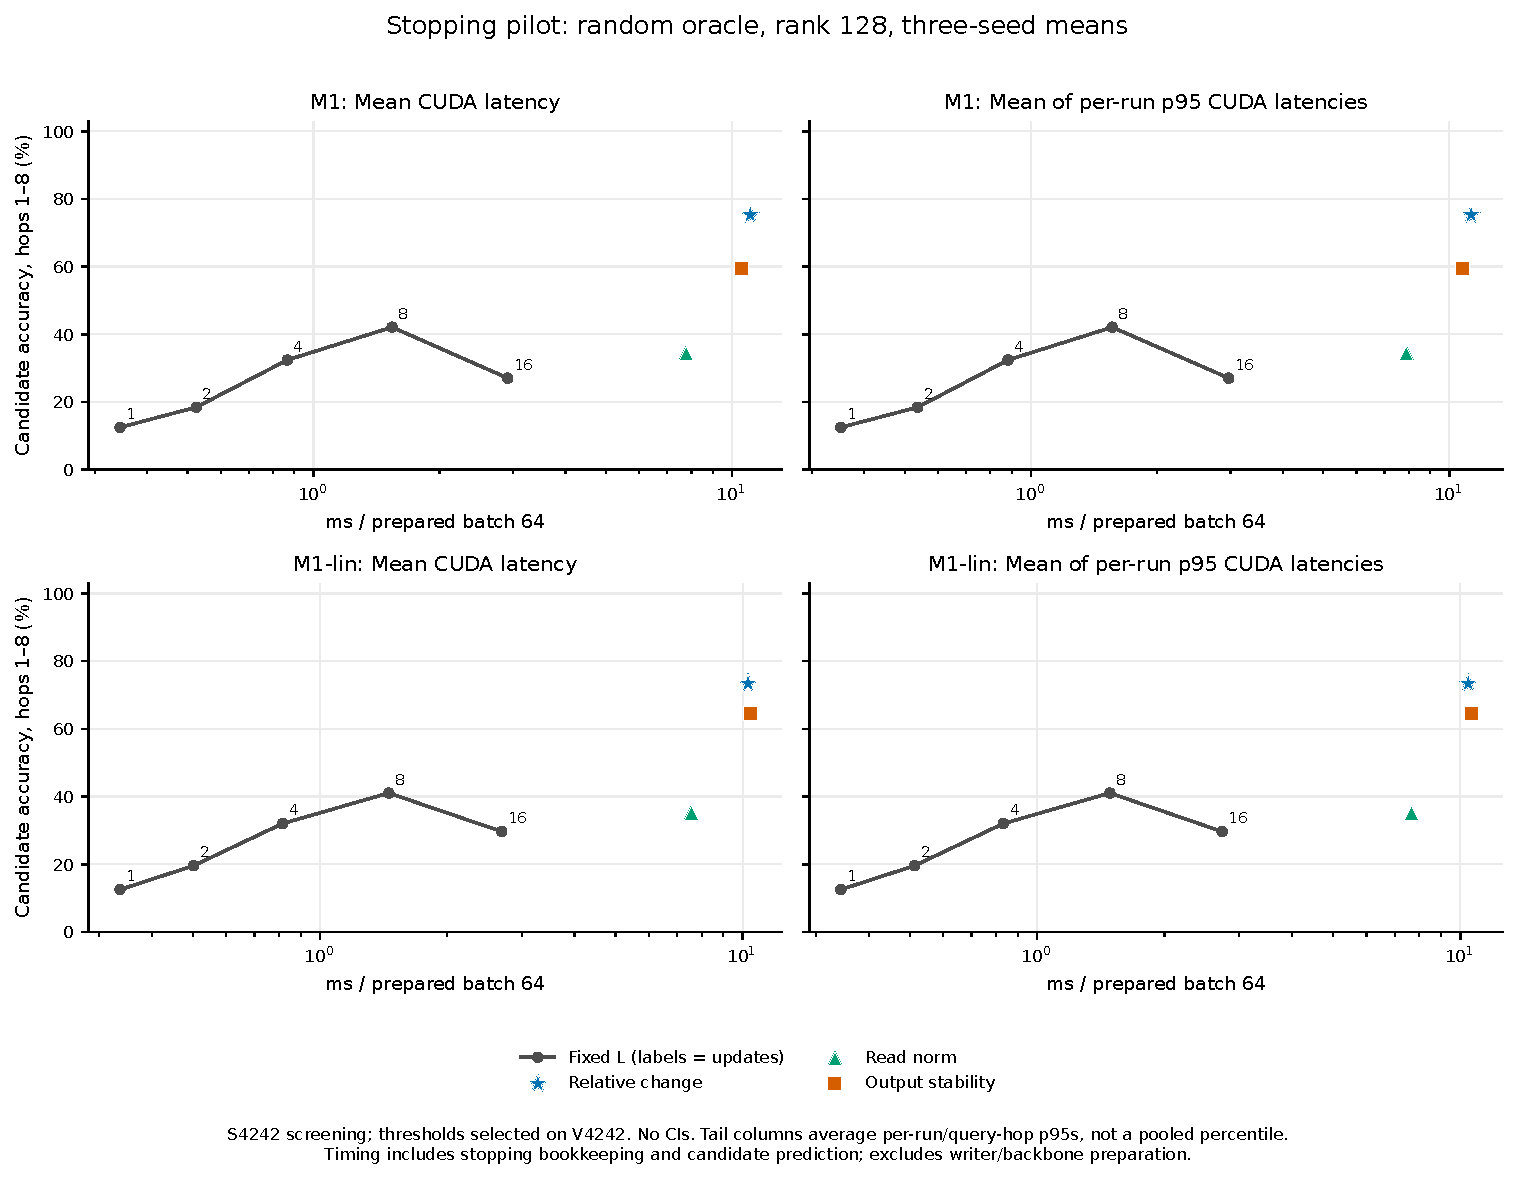
\includegraphics[width=0.96\linewidth]{../figures/stopping_latency.pdf}
\caption{Screening stopping accuracy versus prepared-reader latency, with mean
and exported tail-timing views identified separately. Thresholds are selected on  % H1 H2
validation; plotted screening points have no confidence intervals. Tail columns  % H1 H2
aggregate timing summaries and must not be read as a pooled request-latency
distribution. Fewer steps do not establish a speedup.  % H2 H1 H2
}
\end{figure}

\subsubsection*{Learned post-hoc halting on frozen readers}

P4-S-L trains a separate 3,393-parameter halting head for each frozen reader, using
state and step features with supervised correctness targets. Inputs  % HL1
exclude answer labels, graph distance, correctness, and decoder-confidence features;
the targets still make head training supervised. Reader and writer  % HL1
parameters remain frozen, and one threshold per family is selected on V4242 and
locked before fresh confirmation C999002 (test seed999002, 2,000 episodes).
 The six primary rank32 families are the two activations crossed with  % HL1
factorized joint, frozen factorized, and random-oracle writing.  % HL1

None qualifies: all pass the reach and specificity requirements but fail the
hop1 preservation point threshold H\ensuremath{\geq}\ensuremath{-}1 pp. Here H/\allowbreak{}D compare the learned  % HL1
policy with L1 on hop1/\allowbreak{}hops2-3, and W subtracts the far-hop effect on hops6-8.
 The following intervals are the registered \textbf{99.166667\%} paired  % HL1
episode intervals, adjusted for six primary families, conditional on seeds17/\allowbreak{}29/\allowbreak{}43.
% HL1


{\footnotesize
\setlength{\tabcolsep}{3pt}
\begin{longtable}{W{210}{8}W{411}{8}W{134}{8}W{245}{8}}
\toprule
Writer /\allowbreak{} reader & H, pp (pooled; seeds17/\allowbreak{}29/\allowbreak{}43) & D, pp & W, pp [99.166667\% CI] \\ \addlinespace[3pt]
\midrule \endhead
joint\_fact /\allowbreak{} M1 & \ensuremath{-}33.900; seeds \ensuremath{-}33.850/\allowbreak{}\ensuremath{-}34.950/\allowbreak{}\ensuremath{-}32.900 & +21.583 & +16.517 [15.263, 17.666] \\ \addlinespace[3pt]  % HL1 HL1 HL1
joint\_fact /\allowbreak{} M1-lin & \ensuremath{-}49.150; seeds \ensuremath{-}52.050/\allowbreak{}\ensuremath{-}46.200/\allowbreak{}\ensuremath{-}49.200 & +24.733 & +15.439 [14.026, 16.886] \\ \addlinespace[3pt]  % HL1 HL1 HL1
oracle\_random /\allowbreak{} M1 & \ensuremath{-}15.700; seeds \ensuremath{-}12.350/\allowbreak{}\ensuremath{-}19.250/\allowbreak{}\ensuremath{-}15.500 & +32.508 & +27.975 [26.379, 29.575] \\ \addlinespace[3pt]  % HL1 HL1 HL1
oracle\_random /\allowbreak{} M1-lin & \ensuremath{-}20.850; seeds \ensuremath{-}17.800/\allowbreak{}\ensuremath{-}20.350/\allowbreak{}\ensuremath{-}24.400 & +37.500 & +18.839 [16.947, 20.678] \\ \addlinespace[3pt]  % HL1 HL1 HL1
t1\_frozen\_fact /\allowbreak{} M1 & \ensuremath{-}21.900; seeds \ensuremath{-}22.300/\allowbreak{}\ensuremath{-}20.450/\allowbreak{}\ensuremath{-}22.950 & +9.442 & +6.892 [5.996, 7.774] \\ \addlinespace[3pt]  % HL1 HL1 HL1
t1\_frozen\_fact /\allowbreak{} M1-lin & \ensuremath{-}26.167; seeds \ensuremath{-}26.350/\allowbreak{}\ensuremath{-}25.500/\allowbreak{}\ensuremath{-}26.650 & +10.217 & +7.550 [6.661, 8.447] \\ \addlinespace[3pt]  % HL1 HL1 HL1
\bottomrule
\end{longtable}
}


All eighteen primary per-seed H point estimates also fail preservation.  % HL1
The descriptive unfactorized joint/\allowbreak{}M1 row satisfies the numerical inequalities,
but is outside the primary set and is not a formal qualifying repair.  % HL5
Learned halting exceeds each family’s validation-selected label-free reference in
overall accuracy by +0.883 to +1.615 pp in the four joint\_fact/\allowbreak{}oracle\_random rows,
with positive adjusted intervals; the two frozen-factorized intervals include zero.
 These gains coexist with the preservation failure.  % HL2 HL1 HL2
The label-informed any-step oracle remains 10.250-36.338 pp above the learned policy
in primary families; it upper-bounds selection among the tested frozen candidates,
unlike the distinct true-hop reference. These results reject this  % HL3
head-training and selection scheme as a repair, without ruling out all learned halting.
% HL1

Selected depth is also different from executed work. On confirmation, primary-family
means span 5.306-10.038 selected updates but 12.740-15.995 executed updates.
 If no state crosses the threshold, all 16 updates execute before the  % HL4
earliest maximum-probability state is selected; the post-state feature adds one
memory read beyond the executed updates. In the separate prepared  % HL4
batch64 timing population, primary learned-policy CUDA means are 20.533-25.253 ms
versus 3.072-3.308 ms for fixed L16, with no timing CIs. Those timings  % HL4
include the halting head and bookkeeping, exclude writer/\allowbreak{}backbone preparation,
and do not establish a speedup or end-to-end request cost.  % HL4

\subsubsection*{Hop-1-constrained thresholds and continuation-value heads}

CVH reuses the nine frozen r32 M1 readers of P4-S-L (random-oracle, joint\_fact and
t1\_frozen\_fact writers, seeds17/\allowbreak{}29/\allowbreak{}43) on a new confirmation set C999005 (test seed999005,
2,000 episodes per reader). Arm A1 keeps the P4-S-L head, whose label is that the candidate
argmax at step s is correct, and chooses its threshold on validation under a hop-1 constraint;
arm A2 trains a new head of the same size to predict whether a later read would still lower
the answer’s loss by a 0.25-nat margin. An arm passes if its hops2-3 gain over L1 is at least
3 pp with the interval above 0, its hop-1 change is at least \ensuremath{-}1 pp, and its mean executed
updates are at most 8; the intervals are 99.166667\% (six comparisons) and condition on the
three seeds. Every validation threshold preserved hop 1, so the confirmation set  % CV1
was opened for all three families.  % CV2

Exactly one arm passes: A1 for oracle\_random, with \ensuremath{\theta}=0.10, a hops2-3 gain of +9.950 pp
[9.153, 10.845] over L1, a hop-1 change of +2.883 pp and 1.968 mean executed updates. A halting
head with the correctness label and a hop-1-constrained validation threshold repairs overshoot
for oracle\_random on these frozen readers. The pass is a registered pattern, not  % CV1
a match to fixed-depth reading: the arm’s gain is \ensuremath{-}23.275 pp [\ensuremath{-}24.622, \ensuremath{-}21.942] against fixed L4
and \ensuremath{-}2.908 pp [\ensuremath{-}4.122, \ensuremath{-}1.608] against fixed L16, and the P4-S-L head at its original threshold
(A0) still loses 14.800 pp on hop 1. The A2 head for oracle\_random gains  % CV1 CV4
only +0.492 pp [0.336, 0.675], and both heads for joint\_fact and t1\_frozen\_fact stop at the first
read for every query (\ensuremath{\theta}=0.05, gain +0.000 pp, 1.000 executed updates), so no head repairs
overshoot for the factorized families. No latency claim is made for any arm. The  % CV2
passing arm takes 7.829 ms against 3.108 ms for the fixed 16-update read on a prepared batch of
64, and the four arms whose wall time is below fixed L16 (2.395-2.420 ms against 3.081-3.114 ms)
stop at step 1 and do not pass. The earlier P4-S-L failures stay reported.  % CV3 HL1
No gate depends on CVH.  % CV1

\subsubsection*{Random-depth training with a final-state Jacobian penalty}

JS changes training instead of fitting an exit to frozen trajectories. Its RS
baseline samples one shared-reader depth uniformly from 4-8 per batch; RS+J adds
\(\max(\operatorname{rad}(J(z_L))-.9,0)^2\) with weight 1, averaged over episode/\allowbreak{}query
states at the final training read. Here rad denotes  % JS1 JS6
spectral radius, distinct from the reader scale rho. The ReLU transition Jacobian
uses the next-update gate at reached z\_L, with derivative zero at a zero preactivation;
full numerical eigenvalues are computed in float32, rather than estimated by a power
method. This is a regularizer, not certified eigenvalue arithmetic or  % JS6
an assertion that the reached state is fixed. The two conditions share  % JS6
initialization and data/\allowbreak{}depth RNG streams within seed, then optimize separately;
learned writers may therefore diverge. Both use M1/\allowbreak{}ReLU, rank32,  % JS1
15,000 steps, batch64, and learning rate 0.003.  % JS1

Fresh confirmation C999003 uses test seed999003 and 2,000 episodes, with thresholds
locked on V4242 before test. In this study \textbf{short} means  % JS1 JS4
hops1-3, rather than the earlier reach endpoint’s hops2-3; long remains hops4-8.
 The registered overshoot statistic is S=Acc16\ensuremath{-}Acc4 on short  % JS1 JS3
hops, and DeltaS=S(RS+J)\ensuremath{-}S(RS). All following JS contrast intervals are  % JS1
97.5\% paired episode intervals conditional on the three fixed training seeds; the
per-seed point effects (seeds17/\allowbreak{}29/\allowbreak{}43) follow each pooled value.
% JS1


{\footnotesize
\setlength{\tabcolsep}{3pt}
\begin{longtable}{W{90}{8}W{314}{8}W{304}{8}W{292}{8}}
\toprule
Writer & S(RS), pp [97.5\% CI] & S(RS+J), pp [97.5\% CI] & DeltaS, pp [97.5\% CI] \\ \addlinespace[3pt]
\midrule \endhead
oracle\_random & \ensuremath{-}11.267 [\ensuremath{-}12.356, \ensuremath{-}10.050]; seeds \ensuremath{-}11.900/\allowbreak{}\ensuremath{-}11.017/\allowbreak{}\ensuremath{-}10.883 & \ensuremath{-}2.833 [\ensuremath{-}3.800, \ensuremath{-}1.806]; seeds \ensuremath{-}3.533/\allowbreak{}\ensuremath{-}2.400/\allowbreak{}\ensuremath{-}2.567 & +8.433 [7.483, 9.418]; seeds +8.367/\allowbreak{}+8.617/\allowbreak{}+8.317 \\ \addlinespace[3pt]  % JS1 JS1 JS1
joint\_fact & \ensuremath{-}3.017 [\ensuremath{-}3.789, \ensuremath{-}2.272]; seeds \ensuremath{-}2.800/\allowbreak{}\ensuremath{-}1.950/\allowbreak{}\ensuremath{-}4.300 & \ensuremath{-}1.772 [\ensuremath{-}2.484, \ensuremath{-}1.061]; seeds \ensuremath{-}1.983/\allowbreak{}\ensuremath{-}0.900/\allowbreak{}\ensuremath{-}2.433 & +1.244 [0.222, 2.200]; seeds +0.817/\allowbreak{}+1.050/\allowbreak{}+1.867 \\ \addlinespace[3pt]  % JS1 JS1 JS1
\bottomrule
\end{longtable}
}


Both writers reduce overshoot, with positive DeltaS in every seed, but neither
meets the registered removal criterion: in addition to positive DeltaS and CI,
S(RS+J) must be at least \ensuremath{-}1 pp. Other endpoints expose the cost:  % JS1
% JS2 JS3 JS4


{\small
\setlength{\tabcolsep}{3pt}
\begin{longtable}{W{180}{6}W{412}{6}W{407}{6}}
\toprule
RS+J\ensuremath{-}RS endpoint & oracle\_random, pp [97.5\% CI] & joint\_fact, pp [97.5\% CI] \\ \addlinespace[3pt]
\midrule \endhead
E2: short hops at L4 & +0.789 [0.261, 1.295]; seeds +1.200/\allowbreak{}+0.883/\allowbreak{}+0.283 & \ensuremath{-}0.728 [\ensuremath{-}1.567, 0.067]; seeds \ensuremath{-}0.233/\allowbreak{}\ensuremath{-}0.733/\allowbreak{}\ensuremath{-}1.217 \\ \addlinespace[3pt]  % JS2 JS2
E3: long hops at L16 & \ensuremath{-}5.547 [\ensuremath{-}6.200, \ensuremath{-}4.890]; seeds \ensuremath{-}5.670/\allowbreak{}\ensuremath{-}4.540/\allowbreak{}\ensuremath{-}6.430 & \ensuremath{-}1.443 [\ensuremath{-}1.990, \ensuremath{-}0.933]; seeds \ensuremath{-}0.630/\allowbreak{}\ensuremath{-}1.250/\allowbreak{}\ensuremath{-}2.450 \\ \addlinespace[3pt]  % JS3 JS3
E4: stopped, all hops & \ensuremath{-}1.040 [\ensuremath{-}1.538, \ensuremath{-}0.544]; seeds \ensuremath{-}0.694/\allowbreak{}\ensuremath{-}0.513/\allowbreak{}\ensuremath{-}1.913 & \ensuremath{-}0.677 [\ensuremath{-}1.227, \ensuremath{-}0.115]; seeds \ensuremath{-}0.163/\allowbreak{}\ensuremath{-}0.606/\allowbreak{}\ensuremath{-}1.263 \\ \addlinespace[3pt]  % JS4 JS4
\bottomrule
\end{longtable}
}


Thus longer-walk and stopped accuracy decline for both writers, while joint\_fact’s
L4 short-hop interval crosses zero. RS+J’s stopped  % JS2 JS3 JS4
accuracy is 18.704\%/\allowbreak{}15.879\% for oracle\_random/\allowbreak{}joint\_fact, with 15.938/\allowbreak{}15.028 mean
reads under separately validation-selected relative-change thresholds and cap16;
absolute-rate and read-count CIs are unavailable. This supplies no  % JS4
measured latency advantage.  % JS4

\begin{figure}[htbp]
\centering
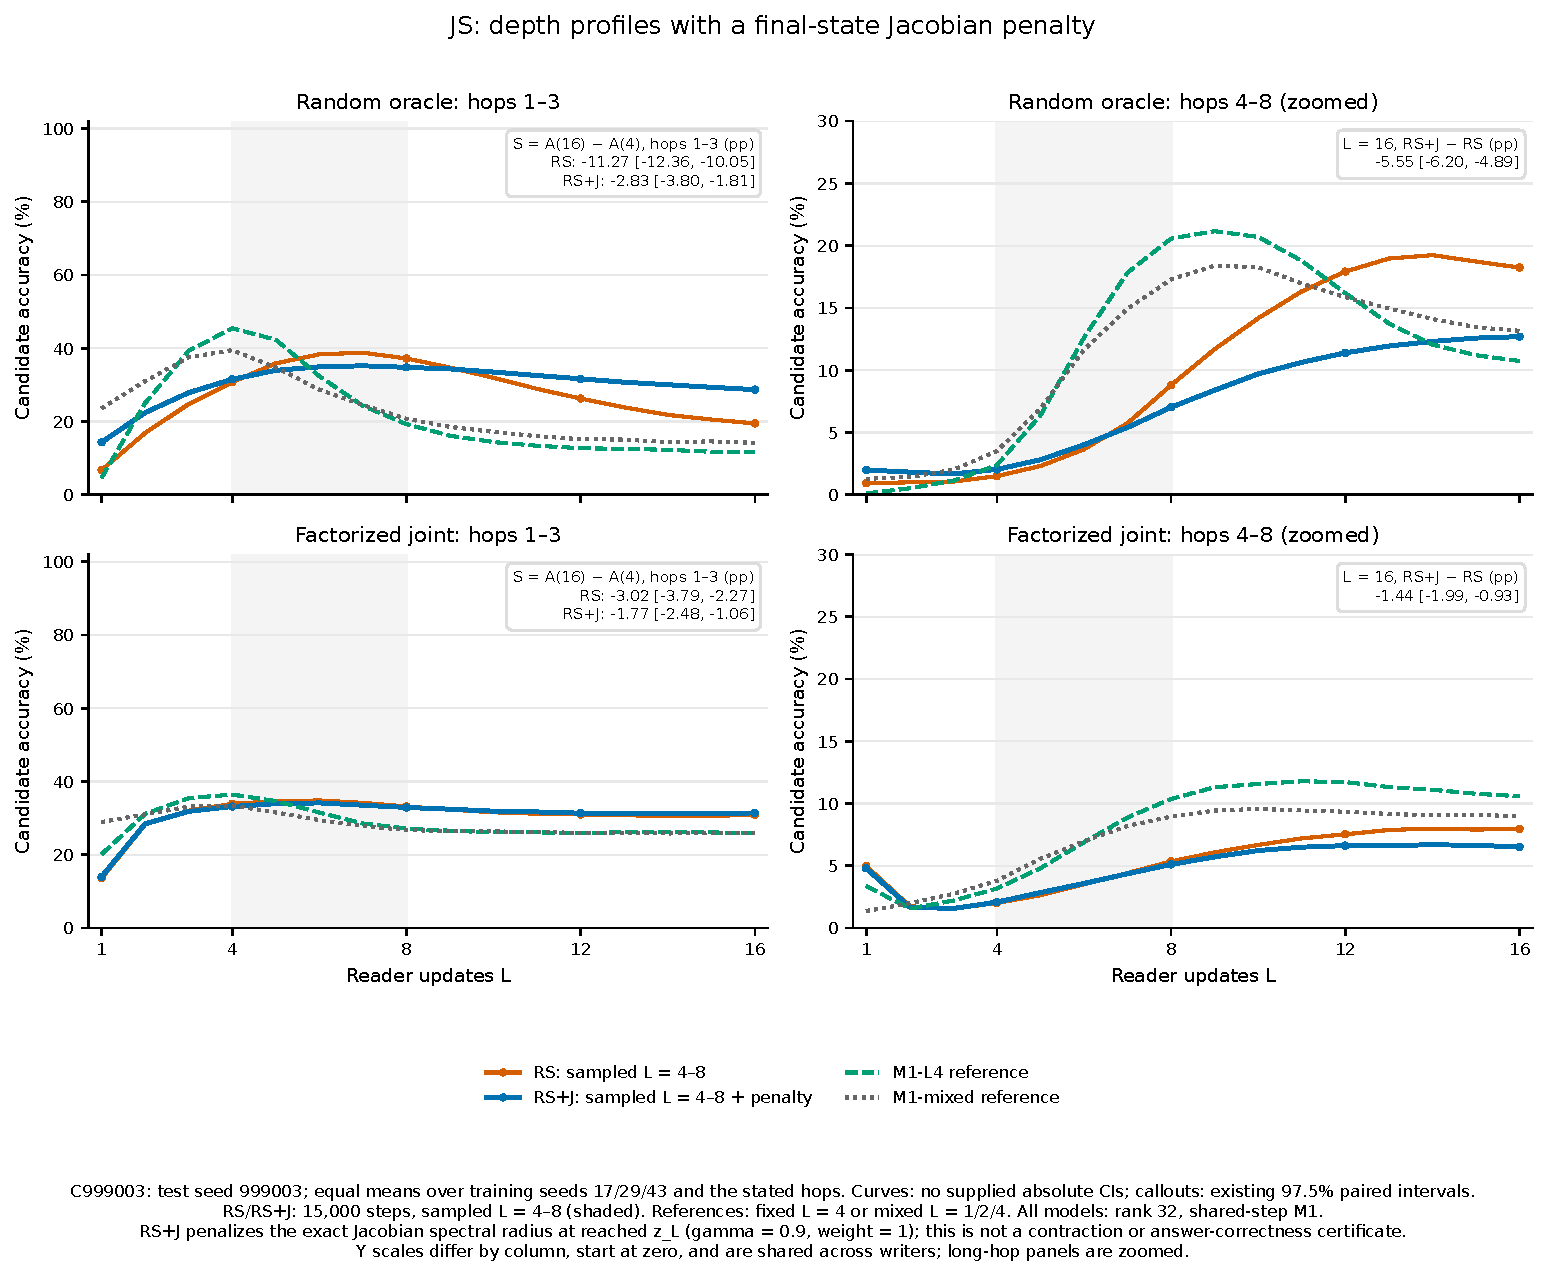
\includegraphics[width=0.96\linewidth]{../figures/js_overshoot.pdf}
\caption{JS C999003: three-seed mean candidate accuracy versus depth, short
hops1-3 and long hops4-8, for RS, RS+J, and unchanged M1-L4/\allowbreak{}M1-mixed references.
 Shading marks RS training depths4-8; absolute  % JS1 JS3 JS5
curves have no supplied CIs, while callouts reuse the released 97.5\% endpoint
intervals. Reduced overshoot retains negative S and costs  % JS1 JS3
longer-walk accuracy. Y scales differ by column; the  % JS1 JS3
long-hop panels are labeled as zoomed views.
}
\end{figure}

The references distinguish random-depth training from the additional penalty.
At L4, random-oracle RS scores below both references on short hops; factorized
RS scores below M1-L4, while its +0.483 pp contrast with M1-mixed has an interval
crossing zero. At L16, RS exceeds both on short hops for both writers. On long hops at L16,  % JS5 JS5
RS exceeds both references for oracle\_random but scores below both for joint\_fact.
 These contrasts change training history; RS+J\ensuremath{-}RS is the comparison  % JS5
that tests adding the penalty.  % JS1 JS5

The descriptive L16 mean radius falls from 1.307 to 1.053 for oracle\_random and
from 0.861 to 0.834 for joint\_fact; only 22.238\% and 92.698\% of RS+J reached states,
respectively, have radius below 1. These summaries pool all hops and  % JS6
three seeds and have no radius CIs. A pointwise radius below 1 at a  % JS6
finite state does not certify global contraction, convergence, terminal
annihilation, or a correct decoded answer. Lower radii coexist here with the
longer-walk and stopped-accuracy losses.  % JS3 JS4 JS6

\subsubsection*{Stay training and a sticky gate}

TSM trains eighteen new r32 M1 readers (oracle\_random and joint\_fact writers, seeds17/\allowbreak{}29/\allowbreak{}43,
15,000 steps, the released learning rate 0.003 with no search): T0 is M1-L4 retrained under the
same code, T1 trains at depth 8 with an answer loss at every step s\ensuremath{\geq}hop, and T2 adds a
content-gated sticky update with two extra parameters. Evaluation uses a new set C999007
(seed999007, 2,000 episodes) at depths 1, 4, 8 and 16, with the released B4 at L1 as the
same-rank reference, and 98.75\% intervals for the four arm-writer comparisons. An arm passes
only if, for both writers, accuracy on hops1-3 differs between L16 and L4 by at most 1 pp
(point), hops4-8 at L8 fall at most 1 pp below T0 (point), and the hops2-3 gain of L4 over B4 at
L1 is at least 3 pp with the interval above 0. No arm passes for either writer. The  % TS1
gain condition holds in all four arm-writer cells (+16.575 and +16.567 pp for oracle\_random
T1 and T2, +16.950 and +21.533 pp for joint\_fact) and the stay condition in one (joint\_fact T1,
\ensuremath{-}0.794 pp), but the far condition fails in all four (\ensuremath{-}11.667, \ensuremath{-}11.780, \ensuremath{-}5.733 and \ensuremath{-}4.553 pp).
 Neither stay training nor the sticky gate removed the overshoot under this protocol;  % TS1
fixed-depth training (M1-L4, B8) remains the remedy found, and the result does not generalise
from one learning rate. Descriptively, hop 1 at L16 falls by 22.5-44.0 pp relative  % TS1
to each arm’s own L1 in all four cells.  % TS2


